
\section{\namee by Examples}
\label{nested:sec:overview}

This section illustrates \namee with an encoding of a family polymorphism
solution to the Expression Problem, and informally presents its salient
features.


%-------------------------------------------------------------------------------
\subsection{The Expression Problem, \namee Style}

The \namee calculus allows us to solve the Expression Problem in a way that is
very similar to \citeauthor{Ernst_2001}'s \textsf{gbeta} solution in \cref{sec:ernst}.
However, the underlying mechanisms of \namee are quite different from those of
\textsf{gbeta}. In particular, \namee features a structural type system in which we can
model objects with records, and object types with record types. For instance, we
model the interface of \lstinline{Lang.Exp} with the singleton record type
\lstinline${ print : String }$. For the sake of conciseness, we use \lstinline{type} aliases
to abbreviate types.
\lstinputlisting[linerange=4-4]{./examples/overview.sl}% APPLY:linerange=PRINT_INTERFACE
Similarly, we capture the interface of the \lstinline{Lang} family in a record,
with one field for each case's constructor.
\lstinputlisting[linerange=8-8]{./examples/overview.sl}% APPLY:linerange=LANG_FAMILY
Here is the implementation of \lstinline{Lang}.
\lstinputlisting[linerange=17-24]{./examples/overview.sl}% APPLY:linerange=LANG_IMPL
We assume several primitive types: fixed width integers \lstinline{Int},
\lstinline{Double} for numeric operations and \lstinline{String} for text
manipulation. A \namee program consists of a collection of definitions and
declarations, separated by semicolon \lstinline{;}.

% - - - - - - - - - - - - - - - - - - - - - - - - - - - - - - - - - - - - - - - -
\paragraph{Adding Evaluation.}
We obtain \lstinline{IPrint & IEval}, which is the corresponding type for \lstinline{LangEval.Exp}, by
intersecting \lstinline{IPrint} with \lstinline{IEval} where
\lstinputlisting[linerange=29-29]{./examples/overview.sl}% APPLY:linerange=EVAL_INTERFACE
The type for \lstinline{LangEval} is then
\lstinputlisting[linerange=34-37]{./examples/overview.sl}% APPLY:linerange=EVAL_PRINT_INTERFACE
We obtain an implementation for \lstinline{LangEval} by merging the existing
\lstinline{Lang} implementation \lstinline{implLang} with the new evaluation
functionality \lstinline{implEval} using the merge operator \lstinline{,,}.
\lstinputlisting[linerange=45-53]{./examples/overview.sl}% APPLY:linerange=EVAL_PRINT_IMPL

% - - - - - - - - - - - - - - - - - - - - - - - - - - - - - - - - - - - - - - - -
\paragraph{Adding Negation.}
Adding negation to \lstinline{Lang} works similarly.
\lstinputlisting[linerange=57-65]{./examples/overview.sl}% APPLY:linerange=LANG_NEG
% \begin{Verbatim}[xleftmargin=10mm,fontsize=\relscale{.80}]
% type LangNeg = Lang & { neg : IPrint -> IPrint }

% implLangNeg : LangNeg
% implLangNeg = implLang ,, implNeg

% implNeg = { neg = \a.{print = "-" ++ a.print } }
% \end{Verbatim}

% - - - - - - - - - - - - - - - - - - - - - - - - - - - - - - - - - - - - - - - -
\paragraph{Putting Everything Together.}
Finally, we can combine the two extensions and provide the missing
implementation of evaluation for the negation case.
\lstinputlisting[linerange=70-80]{./examples/overview.sl}% APPLY:linerange=LANG_FINAL
We can test \lstinline{implLangNegEval} by creating an object \lstinline{e} of expression $-2 + 3$ that is able to print and evaluate at the same time.
\lstinputlisting[linerange=98-100]{./examples/overview.sl}% APPLY:linerange=TEST



%- - - - - - - - - - - - - - - - - - - - - - - - - - - - - - - - - - - - - - - -
\paragraph{Multi-Field Records.} One relevant remark is that
\namee does not have multi-field record types built in. They are merely syntactic
sugar for intersections of single-field record types. Hence, the following is an
equivalent definition of \lstinline{Lang}:
\lstinputlisting[linerange=13-13]{./examples/overview.sl}% APPLY:linerange=LANG_FAMILY2
Similarly, the multi-field record expression in the definition of
\lstinline{implLang} is syntactic sugar for the explicit merge of two
single-field records.
\begin{lstlisting}
implLang : Lang = { lit = ... } ,, { add = ... };
\end{lstlisting}

%- - - - - - - - - - - - - - - - - - - - - - - - - - - - - - - - - - - - - - - -
\paragraph{Subtyping.}
A big difference compared to \textsf{gbeta} is that many more \namee types are related through
subtyping. Indeed, \textsf{gbeta} is unnecessarily conservative~\citep{ernst_hoh}: none of the families is related
through subtyping, nor is any of the class members of one family related to any
of the class members in another family. For instance, \lstinline{LangEval} is
not a subtype of \lstinline{Lang}, nor is \lstinline{LangNeg.Lit} a subtype
of \lstinline{Lang.Lit}.

In contrast, subtyping in \namee is much more nuanced and depends entirely on the
structure of types. The primary source of subtyping are intersection types:
any intersection type is a subtype of its components. For instance, 
\lstinline{IPrint & IEval} is a subtype of both \lstinline{IPrint} and
\lstinline{IEval}. Similarly \lstinline{LangNeg = Lang & NegPrint} is a subtype
of \lstinline{Lang}. Compare this to \textsf{gbeta} where \lstinline{LangEval.Expr} is
not a subtype of \lstinline{Lang.Expr}, nor is the family \lstinline{LangNeg} a
subtype of the family \lstinline{Lang}.

However, \textsf{gbeta} and \namee agree that \lstinline{LangEval} is not a subtype of
\lstinline{Lang}. The \namee-side of this may seem contradictory at first, as we
have seen that intersection types arise from the use of the merge operator, and
we have created an implementation for \lstinline{LangEval} with
\lstinline{implLang ,, implEval} where \lstinline{implLang : Lang}. That
suggests that \lstinline{LangEval} is a subtype of \lstinline{Lang}.
Yet, there is a flaw in our reasoning:
strictly speaking, \lstinline{implLang ,, implEval} is not of
type \lstinline{LangEval} but instead of type \lstinline{Lang & EvalExt}, where
\lstinline{EvalExt} is the type of \lstinline{implEval}:
\lstinputlisting[linerange=41-41]{./examples/overview.sl}% APPLY:linerange=EVAL_INTERFACE2
Nevertheless, the definition of \lstinline{implLangEval} is valid because
\lstinline{Lang & EvalExt} is a subtype of \lstinline{LangEval}.
Indeed, if we consider for the sake of simplicity only the \lstinline{lit}
field, we have that \lstinline{(Int -> IPrint) & (Int -> IEval)} is a
subtype of \lstinline{Int -> IPrint & IEval}. This follows from a standard
subtyping axiom for distributivity of functions and intersections in the BCD system inherited by \namee.
In conclusion, \lstinline{Lang & EvalExt} is a subtype of both \lstinline{Lang}
and of \lstinline{LangEval}. However, neither of the latter two types is a subtype of the other.
Indeed, \lstinline{LangEval} is not a subtype of \lstinline{Lang} as the type
of \lstinline{add} is not covariantly refined and thus admitting the subtyping
is unsound. For the same reason \lstinline{Lang} is not a subtype of \lstinline{LangEval}.


A summary of the various relationships between the language components is shown
in \cref{fig:diagram}. Admittedly, the figure looks quite complex because our
calculus has a structural type system (as often more foundational calculi
do) where more types are related through subtyping, whereas mainstream OO
languages have nominal type systems.



\begin{figure}[t]
  \centering
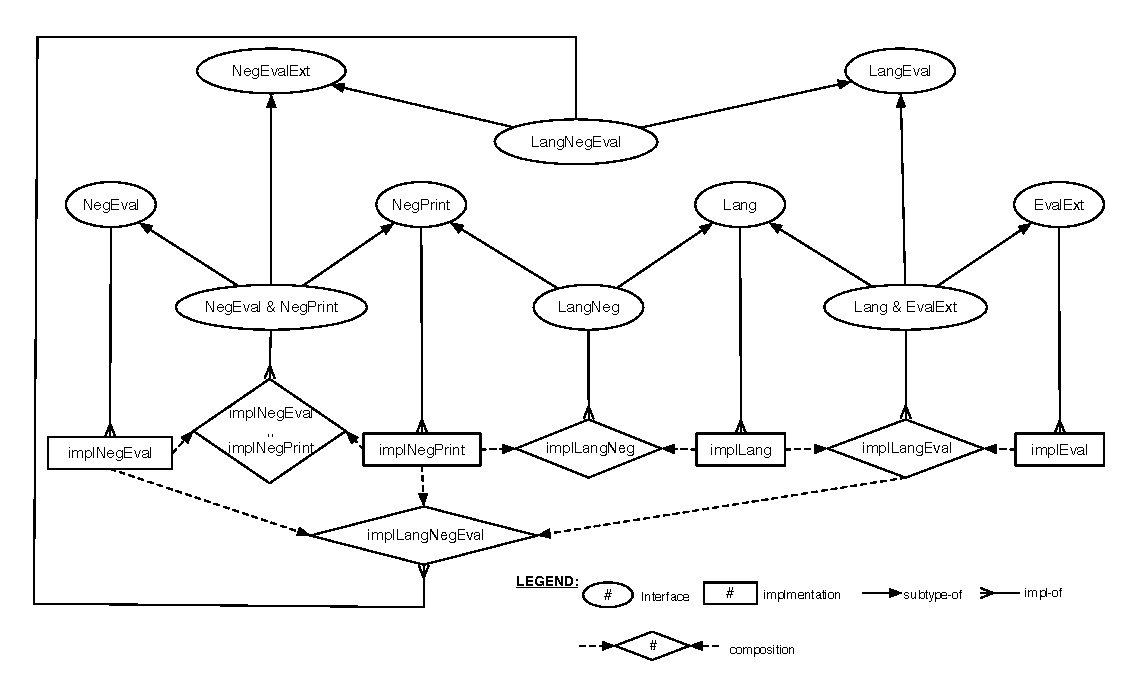
\includegraphics[scale=0.75]{figures/diagram.eps}
\caption{Summary of the relationships between language components}
\label{fig:diagram}
\end{figure}


\paragraph{Stand-Alone Extensions.}
Unlike in \textsf{gbeta} and other class-based inheritance systems, in \namee
the extension \lstinline{implEval} is not tied to \lstinline{LangEval}. In that
sense, it resembles trait and mixin systems that can apply the same extension
to different classes. However, unlike those systems, \lstinline{implEval} can also
exist as a value on its own, i.e., it is not an extension per se.

%-------------------------------------------------------------------------------
% \subsection{Disjoint Intersection Types and Ambiguity}

% The above example shows that intersection types and the merge operator
% are closely related to multiple
% inheritance. Indeed, they share a major concern with multiple inheritance,
% namely ambiguity. When a subclass inherits an implementation of the same
% method from two different parent classes, it is unclear which of the two
% methods is to be adopted by the subclass. In the case where the two parent classes
% have a common superclass, this is known as the \emph{diamond problem}.
% The ambiguity problem also appears in \namee,
% e.g., if we merge two numbers to obtain $\mer{1}{2}$ of type
% $\inter{\mathsf{Int}}{\mathsf{Int}}$. Is the result of $\mer{1}{2} + 3$
% either $4$ or $5$?

% Disjoint intersection types offer to statically detect potential ambiguity and
% to ask the programmer to explicitly resolve the ambiguity by rejecting the
% program in its ambiguous form. In the previous work on \oname, ambiguity is
% avoided by dictating that all intersection types have to be disjoint, i.e.,
% $\inter{\mathsf{Int}}{\mathsf{Int}}$ is ill-formed because the first component
% has the same type as the second.


% Disjoint intersection types ensure unambiguity and conflicts are
% statically detected and manually resolved by programmers. This
% is similar to the trait model.


% Local Variables:
% TeX-master: "../../Thesis"
% org-ref-default-bibliography: ../../Thesis.bib
% End:
